We have analysed various graph properties on five different languages shown in the previous chapter. Results have demonstrated the similarities of languages within the same family, particularly French and German. As well as similarities, their uniqueness could also be seen when comparing the graphs of each language. Especially with languages of a different family. The Indo-European were all more clustered in their graphs but the Japonic and Sino-Tibetan families were much more evenly distributed. Apart from the five languages shown, I have also generated datasets, calculated graph property values and generated the graphs for four more languages. These are Dutch, Spanish, Russian, and Polish. Together with my program, the data and graphs for all nine languages can be found on GitHub via the link:\\

\url{https://github.com/ZakeC1/MathsProject.git}\\

The corpus we used was an extract of a story giving us the initial outlines and correlations for the entire story. Conclusions derived from the analysis of each language can be extrapolated to cover the entire story because the writing style is unique to the author and story. Another reason that this is possible for linguistic analysis is because of the Zipf curve. The Zipf law for languages follow the same curve so vital words in a portion of an extract are most likely to be vital in the entire extract. To see whether or not this is true, I have produced the dataset and graphs for the English translation of the entire story instead of using an extract. Due to the dataset containing over 400 words they are not shown here but can be seen in the GitHub repository provided before. This is the same for graphs since they contain over 400 unique vertices. However, we can see an extract of the top 10 words of highest frequency in Table \ref{table:englishtopcon} along with the same table for the smaller portion of the English story corpus used before. Through comparison, similar values and words remain in the top 10 with only minor altercations. Consequently, by using a respectable sized extract of a text, we are able to generate correlations that can encompass the entire text.

\begin{table}[!htb]
\centering
\begin{subtable}{.45\textwidth}
	\centering
	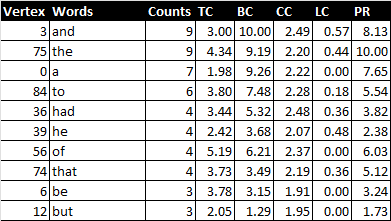
\includegraphics[scale=0.9]{englishtabletop10.png}
	\caption{}
\end{subtable}
\hfill
\begin{subtable}{.45\textwidth}
	\centering
	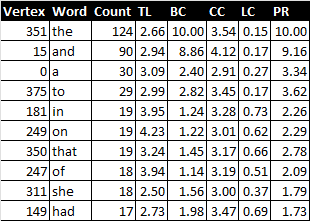
\includegraphics[scale=0.9]{englishfulltabletop10.png}
	\caption{}
\end{subtable}
\caption{Top 10 word of highest frequency based on an (a) extract and (b) full version of the ``Sleeping Beauty" story corpus.}
\label{table:englishtopcon}
\end{table}

Therefore, the study of complex graphical properties such as trophic coherence, various centrality values and clustering have proved beneficially in distinguishing graphs from one another visually. Furthermore, the graph visualisations act as a tool to represent information and unique results. We summarise each graph property and the correlations that were derived from them based on the five languages.

\section{Local Clustering Coefficient}
Local clustering with the linguistic graphs of the five languages analysed seem to correspond to words that would most likely be involved in triples (a 3-cycle). Higher local clustering means that they are more likely involved in a unique directed 3-cycle. However, because of the common reuse of words, there were usually no triples that represented anything unique to the language. This was only realised through the analysis of Japanese and German since they had a larger number of vertices with a high local clustering. Even though the analyse of individual languages did not give a correlation, the combination gave us a correlation that worked for each of the language seen. This was because there was not enough evidence for each individual language to associate the trend to the correlation. A way to improve the usefulness of local clustering in linguistic analysis would be to use specific motifs. Each motif may generate a different visualisation and lead to the generation of unique correlations. Currently, a generic 3-cycle is used for the local clustering calculations so using specific motifs can be further explored.

\section{Betweenness Centrality}
Betweenness centrality was chosen because of its definition to identify the vertices with most control of informational flow. In the context of language analysis, betweenness values corresponded to the most commonly used words in each language which is further proven by the Zipf curve as mentioned in the English analysis. Words of high betweenness tended to be conjunctions and vital words that are necessary in basic sentence structures. High betweenness also meant that the word has a higher occurrence which was verified through the frequencies of the words in every language dataset. Therefore, betweenness centrality remains a good property in linguistic graph analysis to identify the basic building blocks of different languages.

\section{Closeness Centrality}
Closeness centrality determines the vertices that, on average, have the shortest connections to all the other vertices within the graph. For linguistic analysis, closeness centrality correlated to the vertices whom are most likely to isolate the rest of its sentence. This was more evidently seen in French analysis because the French extract contained more unique sentences. Vertices with highest closeness values were second to last words in sentences of the extract that were unique as the removal of these vertices would cause an isolated vertex further down its path. The closeness value would decreases for each unique vertex away from a sentence end. Therefore, closeness centrality is suited to finding the most unique sentences within a corpus.

\section{Page Rank}
The vertices identified with a high page corresponded to the vertices of a high betweenness betweenness with minor differences in some areas of the graph. Page rank is calculated using the number of backlinks a vertex has. Even though the method of calculating page rank is different to betweenness centrality, they both find the vertices that they consider to be important. In terms of linguistics, the important words are the same for both page rank and betweenness. Essentially, without analysing the minor differences each has, they both represent the same thing in a word graph. Therefore, either further study can be done to identify the small differences these have or the use of one for linguistic analysis is continued.

\section{Trophic Level}
Finally, tropic levels are useful in determining the sentence structure and flow in a word graph. Within linguistic analysis, the flow of the sentences were represented by the ranges of trophic levels which were normalised to 0-10, like with the other values. Consequently, they were used consistently as the $y$-positioning downwards from $0-10$ for all graphs. Trophic levels for each vertex represented the average position that they belonged to within a sentence with 0 being the start and 10 at the end. Languages with better sentence structure had more evenly distributed levels due to the fact that their sentence length was not as varied to other languages. This also meant that they have a larger trophic coherence with more distinguishable partitions to the levels in any word graph.

Additionally, through trophic levels visualisation, other graph property values had subsegments of the $y$-range in which they favoured to represent their high values. For example, in the betweenness graphs, the vertices of high betweenness values were centralised on the $y$-axis. Meaning that they appeared most commonly in the middle of sentences. This is grammatically true because words of high importance either appeared as a bridge in a sentence like the conjunction ``and" or are used commonly throughout the sentence. Thus, leading to an average closer to the centre. Another example is the closeness values where most vertices of high values reside on the end of branches of the graph meaning that they have higher trophic levels. Therefore, trophic levels are useful in linguistic analysis to implement structure to the graphs. Additionally, they are most beneficial in larger corpora or extracts with sentences of similar lengths.

\section{Summary}
In conclusion, each graph property have been researched for their use and benefits within a linguistic graph. The calculations for each complex graphical property was also given along with the possible variations which depended on the graph types. I.e. the weights, whether the graph is directed, self-loops, etc. After detailed descriptions of various properties were given, specific ones were transferred and used on different text corpora. The corpus used were translated to different languages in specific language families. This was possible through the use of programming in Python to generate a dataset from a text input (story corpus for each language). The dataset can then be used to formalise a graph so that the calculations for each complex graph property can be calculated from. Furthermore, the values of each property are normalised and applied onto the positions of each vertex to generate a new graph that provides a visual representation for the dataset. Each new graph represents a different complex graph property which achieves the aim of my research. Therefore, the newly generated visualisations of the graph have proven to be useful in linguistic analysis. The graphs are able to highlight key components of interest by showing them as extremes of clusters or as certain outliers. Correlations for each graph property were identified in relation to linguistics. Results found can then be expanded onto a larger dataset to predict the key areas and what words they may correspond to. Proving the usefulness of the graph visualisations which can be taken further into different corpora or different areas entirely.

\section{Future works and Applications}
Some possible applications of graph visualisations and their uses are outlined here. Discussions of different topic areas that may benefit through the use of graph visualisations are also described. These are all areas of interest that explore the use of graph representations in their relative field of study.

\subsection{Lexical Analysis}
As seen in chapter 4, I have explored the linguistic analysis of graphs. However, lexical analysis is an alternative that can be explored. Instead of using entire corpora of different languages, specific words can be studied where each character may derive a certain meaning. An idea for the choice of word would be a word which can have multiple variations such as different tenses or genders. This would be more beneficial in languages such as the Sino-Tibetan language family as they have more emphasis on each individual character and their meaning in each word. Thus, giving the possibility of character analyse rather than word analyse. Additionally, this can act as an improvement for specific language representations such as Japanese and Chinese. Languages such as these do not use words in their sentence structure, but instead use syllables \cite{peng2006temporal} or another variation. This means that the application of graph visualisation on characters or syllables may be more beneficial to the study of these languages.

\subsection{Linguistic Profiling and Predictions}
The graph visualisations can be used as a prediction tool within a similar corpus. Vertices that represent specific words would correspond to a similar location in different visualisations of corpora. This is based on the idea that people can have different writing styles. For example, the graph visualisations generated for a specific author and series for each book would be similar. Furthermore, this means that using the analyse of one book can lead to the same results as the other books. Thus, each author could have their own linguistic profile and can be used to identify which author a graph visualisation closely resembles. The study of different authors can be taken and the comparisons of their graph shapes and property values.

As well as identifying authors or styles of writing, the graph visualisation can be used to analyse new or unknown languages. In theory, this can be accomplished through the comparison of the graphs since languages of the same family produce graphs that have resemblances to one another. If the closest language family is known for an unknown or new language, this language family can be chosen. Once the best language family is chosen, predictions of what components or vertices of the graph represents can be given from the facts of other languages within the same language family. The known graphs can be used as an overlay to the unknown language giving possible meanings and translations for the unknown language. Through comparisons, a predicted translation can be given to the unknown text. Although this may not be entirely accurate, it can give a good outline to the unknown language for further analysis to take place.

Therefore the current works on linguistic analysis and complex graph properties can used to identify writing styles of authors or to assist in the translation of an unknown language.

\subsection{Biology}
Graphical analysis is beneficial in many other areas instead of linguistic analysis. One such area includes Biology since biological networks can be converted into graphs \cite{lesne2006complex}. Once they are in the form of graphs, we can apply graph analyse to generate data values to investigate the biological systems. 

Some examples of biological networks \cite{pavlopoulos2011using} that can be applied to graph analyses are given. The first being metabolic and biochemical networks which studies the metabolism in different organisms. Secondly, Protein-protein interaction (PPI) networks contains information on how different proteins coordinate with each other to accomplish biological processes in cells. Finally, gene regulatory networks (GRNs) which contains information on gene expressions within cells. GRNs can be represented through directed networks and can exhibit patterns and specific motifs giving the possibility of graph analysis. 

A similar idea mentioned in Chapter 1 are the de Bujin graphs which is a representation of DNA sequences. Additionally, a different approach is explored by using spectral clustering to identify certain genetic ancestry in the paper by Lee, Luca, Klei, Devlin and Roeder \cite{lee2010discovering}. They analyse genetic ancestry to identify the genes responsible for certain complex diseases and they assess single-nucleotide polymorphism (SNP) genotypes for any association with the various diseases. Therefore, since many biological systems can be represented with graphs, the same procedures can be undergone to identify any correlations in the biological networks instead of linguistic analysis. Discovering potential correlations may prove beneficial to the scientific field and medical advances in curing diseases.

Another such area is the field of neuroscience. The brain \cite{de2014graph} can be regarded as a complex network of neurons where each vertex represents units or specific regions, and the edges represents the links or connections between them. Analysis of neurological diseases such as schizophrenia, dementia and Alzheimer's can be used to generate their relative graph visualisations. These visualisations can be studied further to find common links and correlations within each neurological disease so that action could be taken if early signs of similar correlations are found within a healthy brain. In the medical field, early discovery of these neurological diseases are crucial in taking steps in the early stages so that ????for somebody's recovery which can alter their lives. A similar idea was studied based on detecting changes in the brain which has Alzheimer's using graph theory \cite{10.1093/braincomms/fcaa129}.\\


\noindent In conclusion, graph theory is crucial in representing various types of information in the real world from social groups to the complex structures of the genes and brain. Through the use of different graph properties, different correlations may surface each leading to their own beneficial discovery. Many subject areas can be represented as graph construct which means that they can undergo similar graphical analysis and visualisations. Therefore, linguistic analysis based on complex graph properties is just one of many possible branches to the graph analysis undertaken.